
\documentclass{beamer}
\usepackage{hyperref}
\usepackage{graphicx}
\usepackage[outercaption]{sidecap}
\usepackage[style=verbose,autocite=footnote,citestyle=authoryear]{biblatex}
\addtobeamertemplate{footnote}{\vspace{-6pt}\advance\hsize-0.5cm}{\vspace{6pt}}
\makeatletter
\renewcommand*{\footnoterule}{\kern -3pt \hrule \@width 2in \kern 8.6pt}
\makeatother

\usetheme{Frankfurt}
\addbibresource{references.bib}

\graphicspath{ {images/} }

\title{Assistive Device to map and interpret the local scene for imparting Spatial Awareness in Visually Impaired People}

% A subtitle is optional and this may be deleted
%\subtitle{Optional Subtitle}

\author{A.~Parmar \and P.~Sinha}

\institute[University of Delhi]
{
  Design Innovation Centre\\
  University of Delhi}

\date{September 16, 2015}

\subject{Theoretical Computer Science}

\pgfdeclareimage[height=1cm]{university-logo}{Logo.png}
\logo{\pgfuseimage{university-logo}}

% Delete this, if you do not want the table of contents to pop up at
% the beginning of each subsection:
\AtBeginSection[]
{
  \begin{frame}<beamer>{Outline}
    \tableofcontents[currentsection,currentsubsection]
  \end{frame}
}

% Let's get started
\begin{document}

\begin{frame}
  \titlepage
\end{frame}

\begin{frame}{Outline}
  \tableofcontents
  % You might wish to add the option [pausesections]
\end{frame}

\section{Introduction}
\subsection{Statement of Problem}
\begin{frame}{Background}
  \begin{itemize}
  \item {
    Visually impaired people confront a number of challenges in their daily life - from figuring out if they are at the correct bus stop to reading the label on their soft drink bottle.
  }
  \item {
    Navigation, for instance, is very difficult for a person and prevents the user from moving independently or walk safely.
  }
  \end{itemize}
\end{frame}
\begin{frame}{Current Development}
  \begin{itemize}
  \item {
    Through the global penetration of Smart Phones, access to Navigation Services that are assisted though GPS are available very easily and are cost affective.
  }
  \item {
    However, the instructions provided by the Navigation Services require personal judgement of the user to follow. This includes avoiding obstacles that are encountered on the way, staying on the sidewalk and in correct direction and so on. This is not an easy task for a visually impaired person.
  }
  \item {
    The services also fail to work in an indoor environment.
  }
  \end{itemize}
\end{frame}

\subsection{Proposed Solution}
\begin{frame}{Local Spatial Awareness}
  \begin{itemize}
  \item {
    We propose that increasing the local spatial awareness is a key solution to this problem, and would help the visually impaired people gain more self-reliance.
  }
  \end{itemize}
\end{frame}
\begin{frame}{Deliverables}
  Through this project, we aim to build a wearable device in the form factor of an spectacle that combines information obtained from a 3D Depth Sensor, Inertial Measurement Unit and an Smartphone to do the following:
  \begin{itemize}
  \item {
    Attempts to identify, classify, and interpret the local scene in real time
  }
  \item{
   Communicates the interpreted scene meta data to a smartphone companion app, which combines this information with user intent and communicates the highlighted features of the scene though voice or haptic output.
  }
  \item{
    In case of an ongoing navigation event, the device will combine the navigation information with the scene metadata and give high resolution navigation information that will help the user avoid obstructions.
  }
  \item{
    In case of an indoor scene, the device will try to identify as many objects as possible with metadata obtained through the internet.
  }
  \end{itemize}
\end{frame}

% IMU DATA Information
\section{Inertial Measurement Unit}
\subsection{Introduction}
\begin{frame}{Introduction}
  \begin{itemize}
  \item {
    An Inertial Measurement Unit is a set of various devices that determine the motion of the Unit and hence the device it is pivot to.
  }
  \item{
    An IMU may contain an Accelerometer, Gyroscope, Magnetometer, GPS, Pressure Sensor etc.
  }
  \end{itemize}
\end{frame}
\begin{frame}{9 Degrees of Freedom}
  \begin{itemize}
  \item{
    An accelerometer measures the acceleration in a particular axis.
  }
  \item{
    A gyroscope measures the rate of rotation in a particular axis.
  }
  \item{
    A magnetometer (also known as a digital compass) measures the magnitude of magnetic field in a particular axis.
  }
  \item{
    Through a combination of these three devices, in the three orthogonal axes, it is possible to accurately reproduce the motion of an object the array is pivoted to.
  }
  \end{itemize}
\end{frame}
\subsection{Motion Tracker}
\begin{frame}{Sensor Array}
  \begin{itemize}
  \item{
    For motion tracker prototype, we used MPU-9250\footnote{MPU 9250 (Invensense \url{http://www.invensense.com/products/motion-tracking/9-axis/mpu-9250/})} as the Inertial Measurement Unit and Arduino as the System Processor.
    \begin{figure}[h]
    \centering
    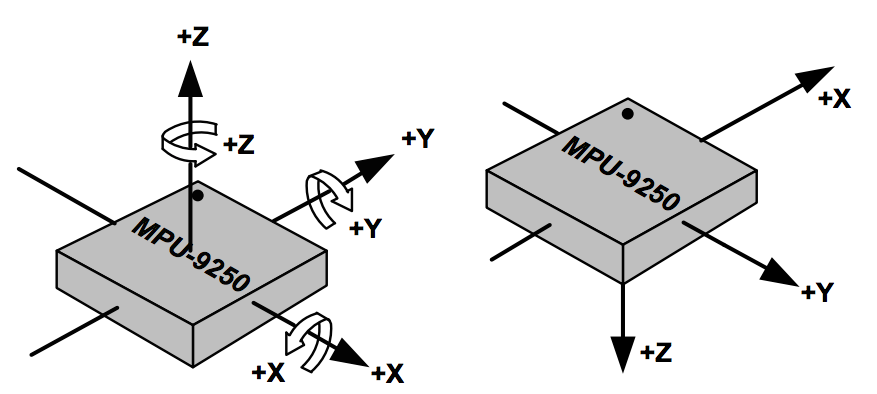
\includegraphics[width=0.5\textwidth]{axes_MPU9250.png}
    \caption{Orientation of the orthogonal axes on the MPU-9250. Left: Accelerometer, Gyroscope; Right: Magnetometer.}
    \end{figure}
  }
  \item{
    IMU was interfaced as a slave I2C device to the System Processor.
  }
  \end{itemize}
\end{frame}
\begin{frame}{Prototype Build}
  \begin{itemize}
  \item{
    We built an Arduino Shield which includes MPU-9250 IMU, SD Card (for on-board data logging), and a 8 bit motion class tagging switch.
    \begin{figure}[h]
      \centering
      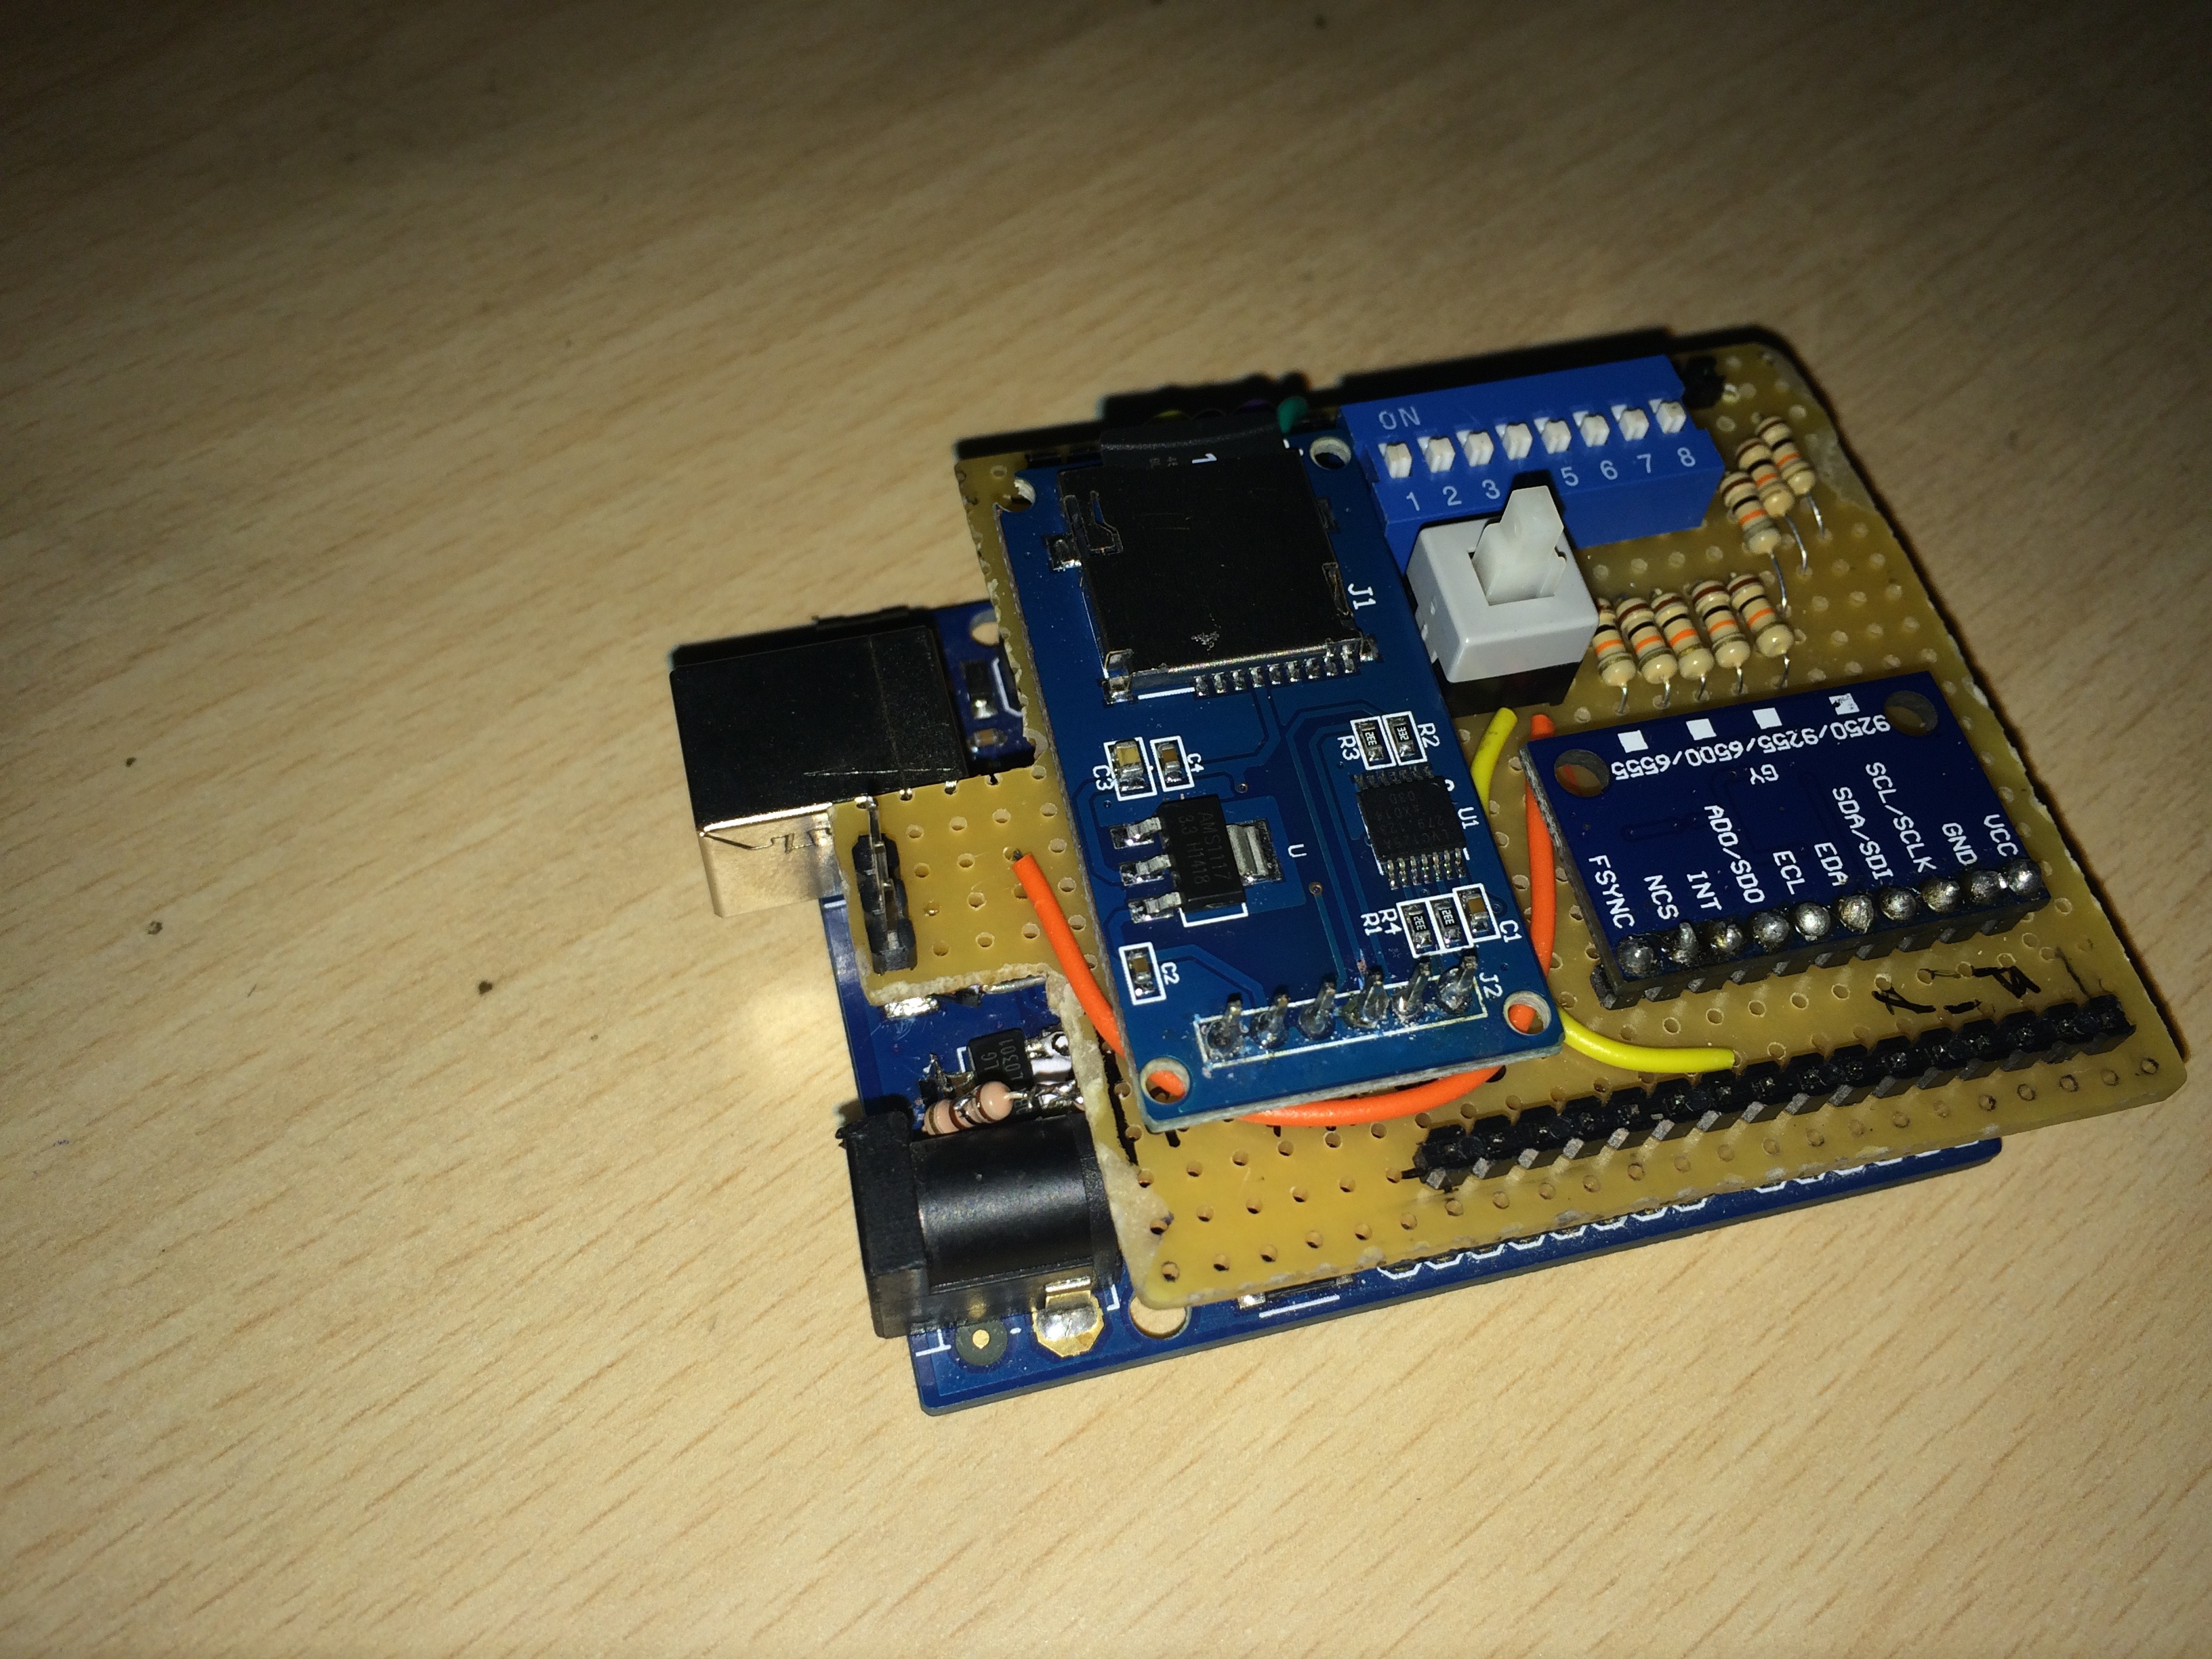
\includegraphics[width=0.4\textwidth]{IMG_2718.jpg}
      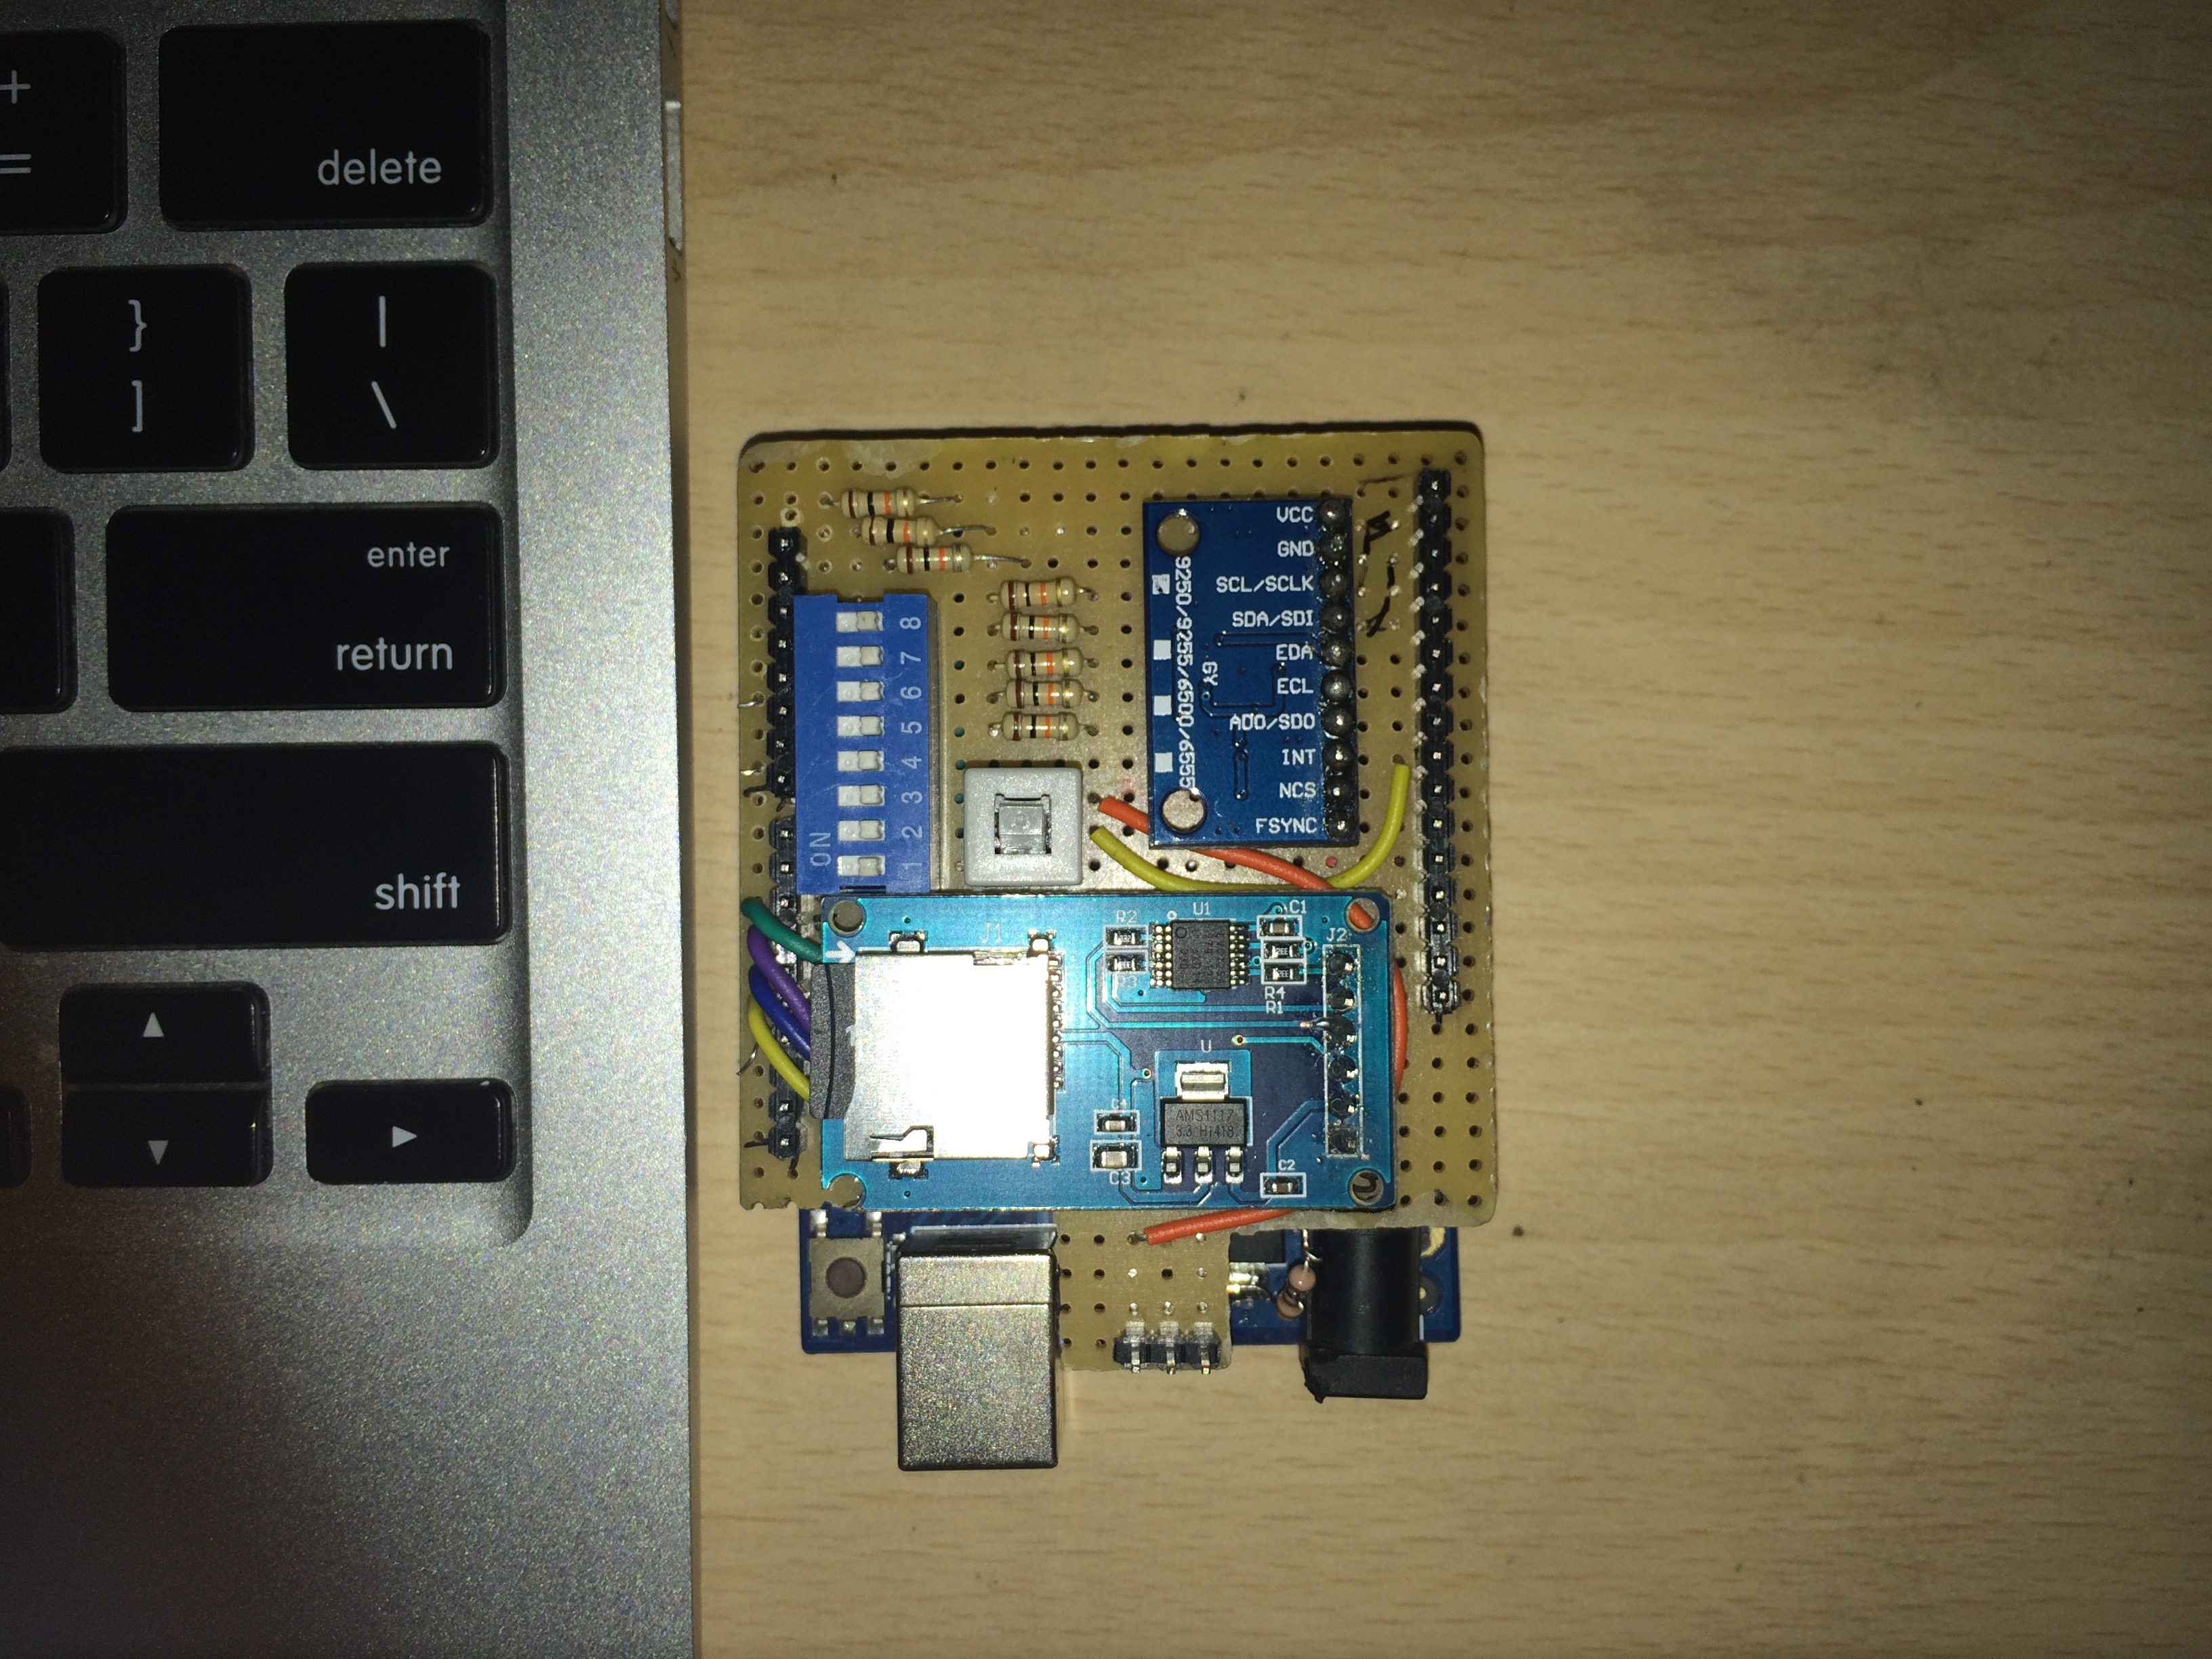
\includegraphics[width=0.4\textwidth]{IMG_2720.jpg}
    \end{figure}
  }
  \item{
    We also wrote a command - line tool to offload, and stream data from tracker.
  }
  \end{itemize}
\end{frame}
\subsection{Sensor Data Fusion}
\begin{frame}{Attitude and Heading Reference System}
  \begin{itemize}
  \item{
    Data from the three axes of the accelerometer, gyroscope and magnetometer are fused to get the Attitude and Heading of the device: Yaw, Pitch and Roll.
  }
  \item{
    Quaternion filter was implemented as an orientation filter\footnotemark.
  }
  \end{itemize}
\footcitetext{Madgwick2011}
\end{frame}
\subsection{Logging and Visualisation}
\begin{frame}{Time-Series Database}
  \begin{itemize}
  \item{
    We used InfluxDB for efficient logging and retrieval of sensor data for further processing.
  }
  \item{
    The sensor data can be sent to the server through UDP channel over WiFi, though USB, or can be logged onto an on-board MicroSD card.
  }
  \end{itemize}
\end{frame}
\begin{frame}{Data Visualisation}
    \begin{figure}[h]
    \centering
    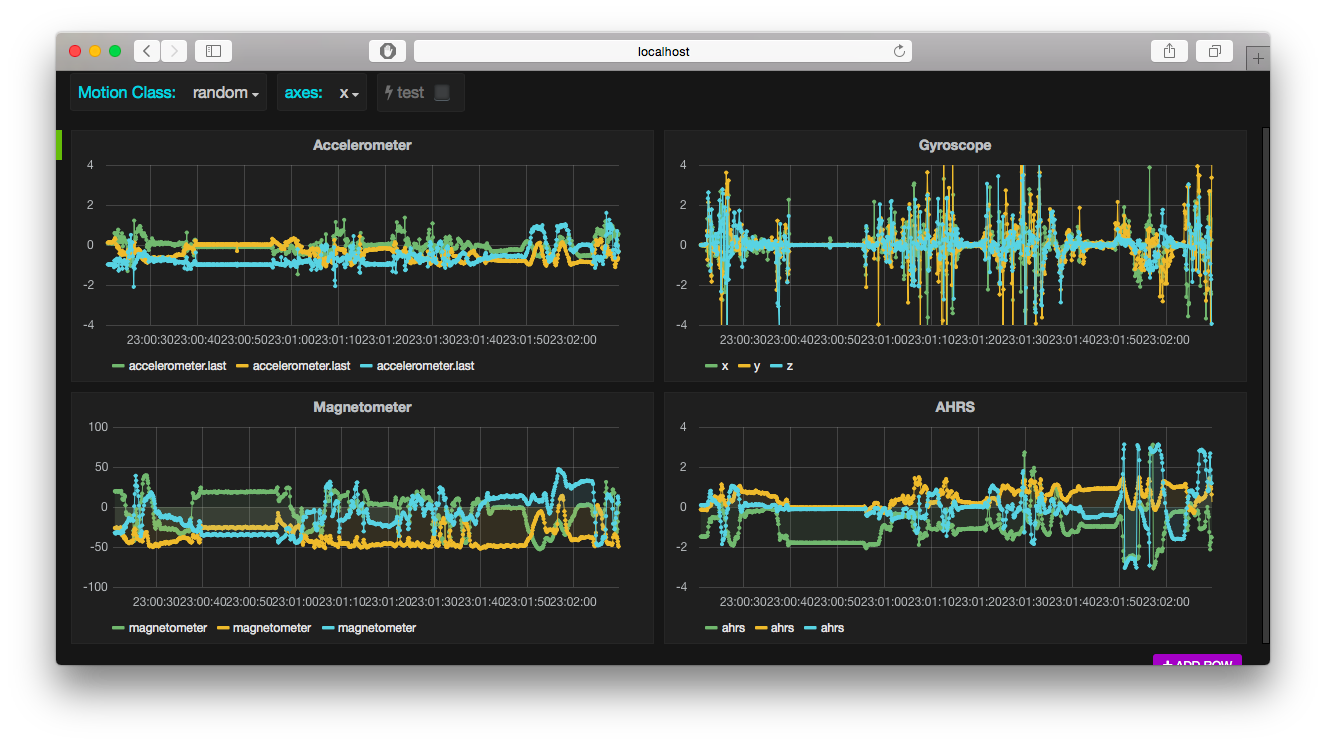
\includegraphics[width=0.9\textwidth]{grafana_dbd.png}
    \caption{Example of the Dashboard showing the raw data samples as well as the "fused" AHRS data.}
    \end{figure}
\end{frame}
\begin{frame}{Motion Visualisation}
    \begin{figure}[h]
    \centering
    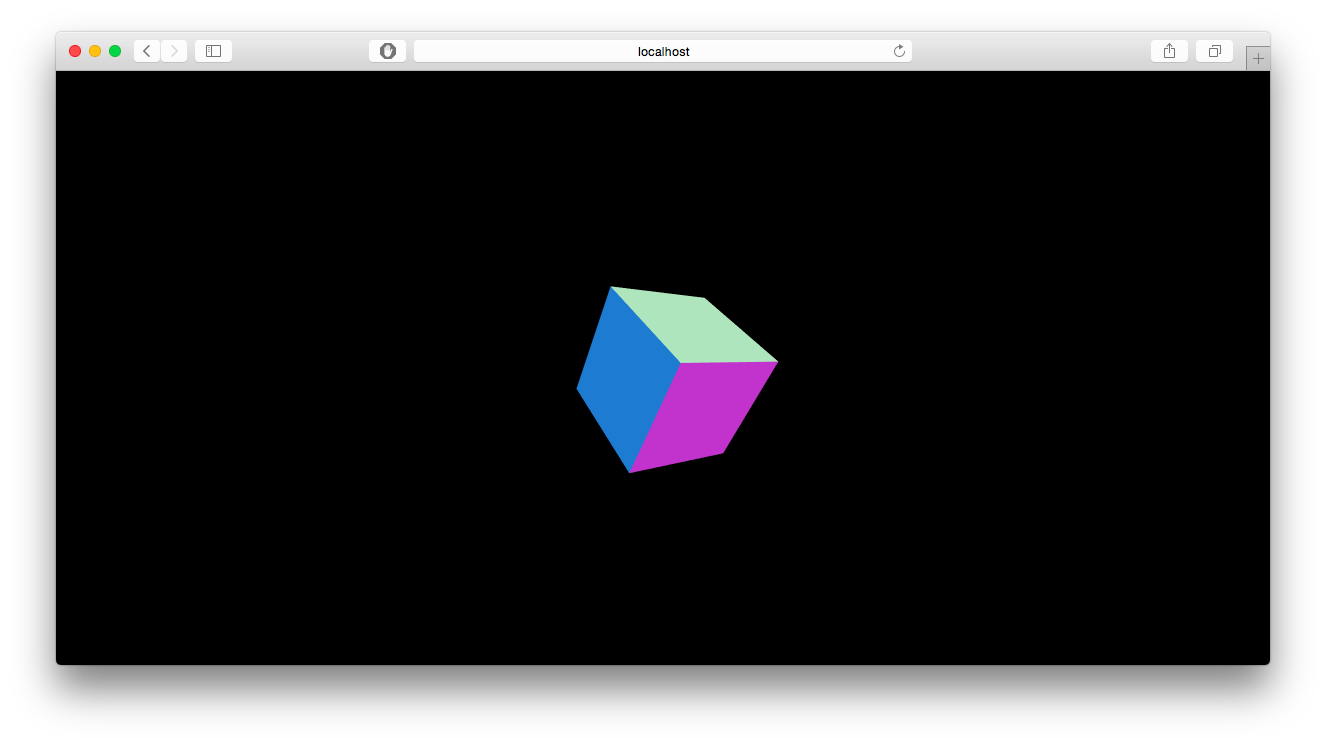
\includegraphics[width=0.9\textwidth]{ahrs_js.png}
    \caption{Real-time visualisation of device motion.}
    \end{figure}
\end{frame}
\section{Human Motion Tracking}
\subsection{Introduction}
\begin{frame}{Introduction}
  \begin{itemize}
  \item {
    Human Motion Tracking refers to the process of inferring the current state of the user.
    This includes tracking if the user is Walking, Running, Climbing the Stairs, is Stationary, etc.
  }
  \item{
    The output from the Human Motion Tracking algorithms are used for providing contextually relevant behaviour in other application or services.
  }
  \item{
    We here investigate the usage of Accelerometer data to infer the motion.
  }
  \end{itemize}
\end{frame}
\subsection{Methodology}
\begin{frame}{Preliminary Investigation}
  \begin{figure}[h]
  \centering
  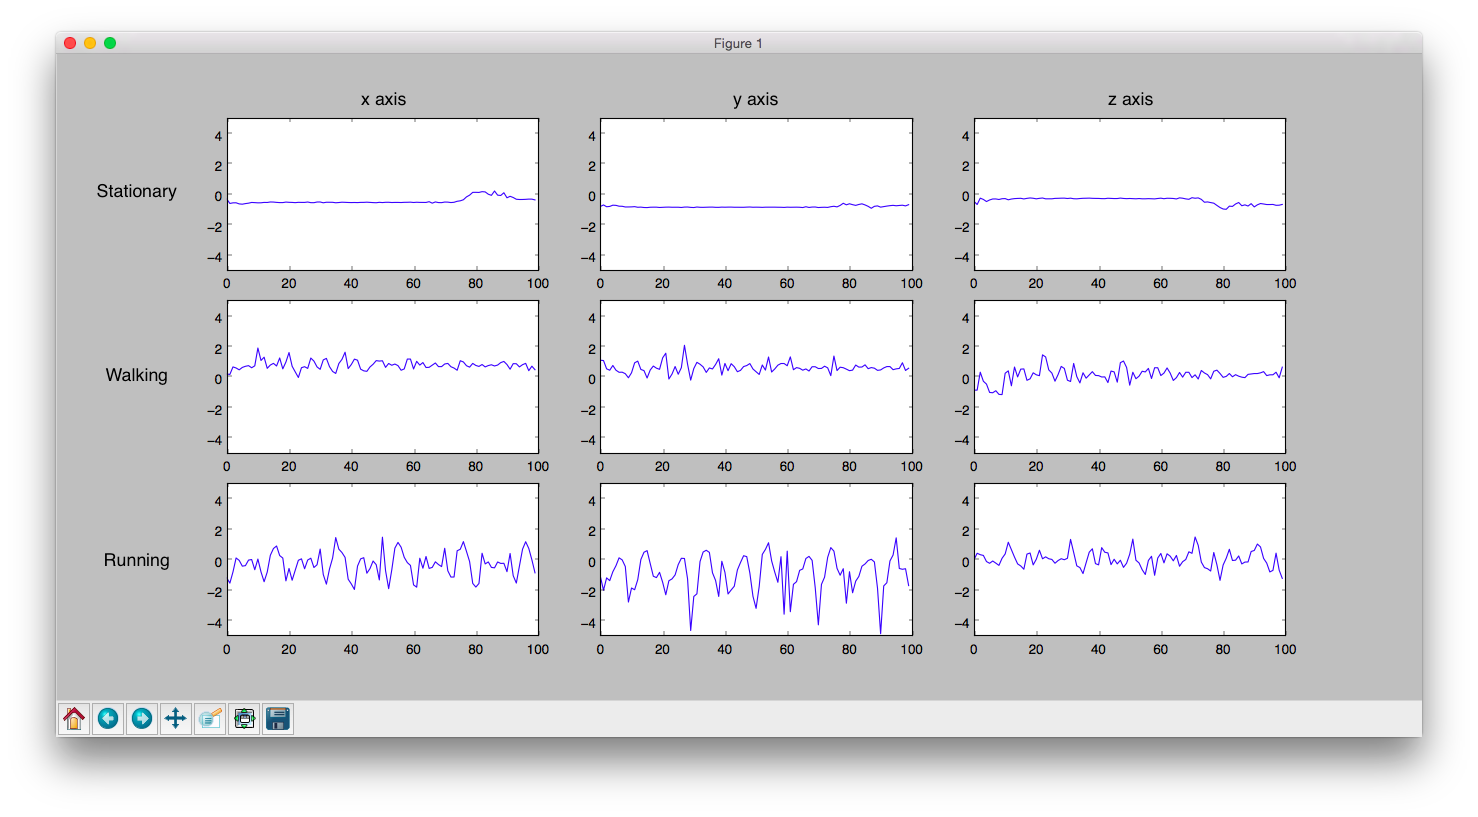
\includegraphics[width=0.7\textwidth]{raw_data.png}
  \caption{Random data sample taken from each motion class.}
  \end{figure}
  \begin{itemize}
  \item {
    To qualitatively represent this data through a feature vector, we have to keep into the consideration that the order in which the values are arriving is important, hence a buffer window is needed.
  }
  \end{itemize}
\end{frame}
\begin{frame}{Wave Chunks}
  \begin{itemize}
  \item {
    To further process the data, we divide the wave into overlapping chunks of length $16$. Overlapping is required to preserve all possible data patterns.
  }
  \item {
    We do this by having a buffer of length $16$ (a window). Initially the buffer head is aligned to $0^{th}$ element of the wave, and then sequentially moved forward by one.
  }
  \item{
    During each iteration, we store the buffer content for further processing. The content is stored as a wave chunk of length 16.
  }
  \end{itemize}
\end{frame}
\begin{frame}{Feature Generation - Periodic Nature}
  \begin{itemize}
  \item{
    We observe that the motion has a Periodic nature. To naively quantify some periodic nature in a wave chunk, we fit the chunk into a sine wave, given by:
    $$ y = a\sin(bx + c) + d $$
    Where, $a$ is Amplitude, $b$ is Phase, $c$ is Phase Shift and $d$ is Vertical Shift.
    This reduces a $n$ length wave chunk to a four dimensional vector: $ P_{axis} = [\begin{smallmatrix}a & b & c & d\end{smallmatrix}]$.
  }
  \item{
    We obtain $p_{axis}$ for the $x, y, z$ axis to get:
    $$ P = \begin{pmatrix}
                a_x & b_x & c_x & d_x \\
                a_y & b_y & c_y & d_y \\
                a_z & b_z & c_z & d_z
           \end{pmatrix}$$
  }
  \end{itemize}
\end{frame}
\begin{frame}{Feature Generation - Periodic Nature}
  \begin{itemize}
  \item{
    The feature vector $P$ obtained is further reduced to its qualitative parameters by selecting a $3\times3$ submatrix from $P$:
    $$ Q = \begin{pmatrix}
                a_x & b_x & c_x \\
                a_y & b_y & c_y \\
                a_z & b_z & c_z 
           \end{pmatrix}$$
  }
  \item{
    We obtain the eigenvalues associated with $Q$ to get
    $$ R = \begin{pmatrix}e_a & e_b & e_c\end{pmatrix}
    $$
  }
  \item{
    We use $R$ as a feature for the given wave chunk. It should be noted that however long the chunk be, this feature's length remains three.
  }
  \end{itemize}
\end{frame}
\begin{frame}{Supervised Learning through Support Vector Machine}
  \begin{itemize}
  \item{
    We built a database of motion data captured while a human subject was "Stationary", "Walking", and "Running" to test the feature validity.
  }
  \item{
    We obtained accelerometer data for each Motion Class for all the three axes. The overlapping window length was set to 16.
  }
  \item{
    We created feature vector for the wave chunks and trained the SVM on a Gaussian and 3 Degree Polynomial Kernels.
  }
  \end{itemize}
\end{frame}
\subsection{Results}
\begin{frame}{Human Motion Tracking}
    \begin{itemize}
    \item {
      We were able to successfully classify between the three basic Motion Classes. (Performance not quantified yet.)
    }
    \item {
      To get better result, we require to collect longer, more refined data set for training.
    }
    \end{itemize}
\end{frame}

\section{Next Steps}
\subsection{Object recognition in 3D Point Cloud Data}
\begin{frame}{3D Point Cloud Data}
  \begin{itemize}
  \item {
    3D Point Cloud is a collection of touples containing the $(x, y, z)$ coordinates of a voxel in a 3D space.
  }
  \item {
    A point cloud image contains depth information, from which a 3D model of the scene can be re-constructed.
  }
  \end{itemize}
\end{frame}
\begin{frame}{Proposed Recognition Methodology Overview}
  \begin{itemize}
  \item {
    We collect normalised point clouds of template objects and shapes in a simulated environment.
  }
  \item {
    We train an un-supervised classifier (eg. ANN, k-Means) to classify between the template objects.
  }
  \item {
    In a complex scene, containing the combination of the template objects and some foreign objects, we first cluster the point clouds.
  }
  \item {
    The clustered point clouds are then classified though the template classifier.
  }
  \end{itemize}
\end{frame}

\subsection{Context recognition}
\begin{frame}{Introduction}
  \begin{itemize}
  \item {
    The scene data collected though object detection is then used to identify the Contexts of the detected objects.
  }
  \item {
    Through the context information, using Bag of Words classifier, we can generate a scene description.
  }
  \item {
    The scene description effectively solves a large portion of the Problem Statement.
  }
  \end{itemize}
\end{frame}

\section*{Summary}

\begin{frame}{Summary}
  \begin{itemize}
  \item {
    Problems faced by visually impaired people, and proposed a solution.
  }
  \item {
    Usage of IMU to identify and classify Human Motion, and AHRS.
  }
  \item {
    Proposed methodology for Point Cloud Data classification.
  }
  \end{itemize}
\end{frame}

\end{document}
